% ============================================================
%  Cram — Architecture Diagrams
%  Paste into Overleaf. Compile with pdfLaTeX.
% ============================================================
\documentclass[12pt,a4paper]{article}
\usepackage[margin=2cm]{geometry}
\usepackage{tikz}
\usepackage{pgfplots}
\pgfplotsset{compat=1.18}
\usepackage{pgf-pie}
\usetikzlibrary{
  arrows.meta, shapes.geometric, shapes.misc,
  fit, positioning, backgrounds, calc,
  decorations.pathreplacing, matrix, shadows
}
\usepackage{xcolor}
\usepackage{caption}
\usepackage{float}

% ---- palette ---------------------------------------------------
\definecolor{ink}    {HTML}{23272E}
\definecolor{blue}   {HTML}{2F5C8F}
\definecolor{bluesoft}{HTML}{E3ECF6}
\definecolor{yellow} {HTML}{FFE066}
\definecolor{ysoft}  {HTML}{FFF3C4}
\definecolor{green}  {HTML}{3F7D58}
\definecolor{red}    {HTML}{B4472A}
\definecolor{paper}  {HTML}{FAF6EE}
\definecolor{card}   {HTML}{FFFDF9}
\definecolor{inksoft}{HTML}{6B7280}
\definecolor{inkfaint}{HTML}{9AA1AB}

% common node styles
\tikzset{
  box/.style    = {draw=ink, thick, rounded corners=6pt,
                   fill=card, minimum height=1cm,
                   text width=2.8cm, align=center, font=\small},
  wbox/.style   = {box, text width=3.5cm},
  accent/.style = {box, fill=bluesoft, draw=blue, text=blue},
  warn/.style   = {box, fill=ysoft,    draw=yellow!80!black},
  good/.style   = {box, fill=green!10, draw=green, text=green!30!black},
  bad/.style    = {box, fill=red!10,   draw=red,   text=red!70!black},
  arr/.style    = {-{Stealth[length=6pt]}, thick, ink},
  darr/.style   = {arr, dashed},
  labl/.style   = {font=\footnotesize\itshape, text=inksoft},
  title/.style  = {font=\bfseries\large, text=ink},
  sub/.style    = {font=\small, text=inksoft},
}

\begin{document}
\pagestyle{empty}

% ==============================================================
% DIAGRAM 1 — End-to-End System Overview
% ==============================================================
\begin{figure}[H]
\centering
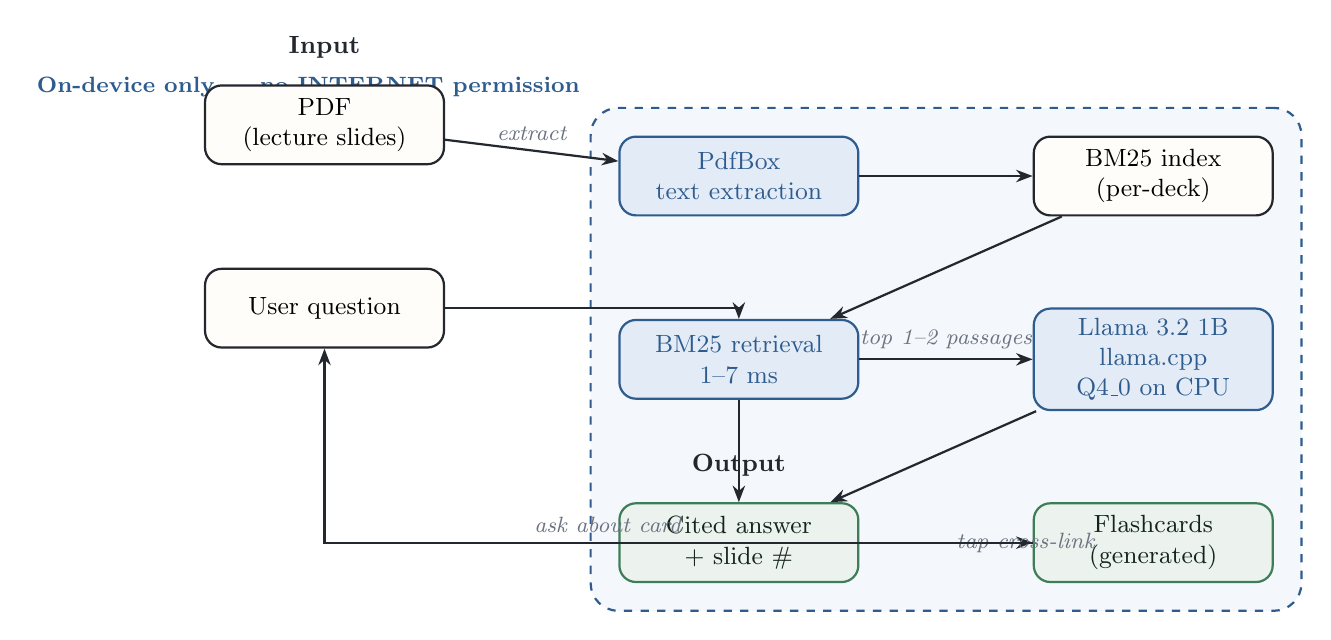
\begin{tikzpicture}[node distance=1.3cm and 1.6cm]

  % --- left column: input ---
  \node[box] (pdf)  {PDF\\\small(lecture slides)};
  \node[box, below=of pdf] (ask) {User question};

  % --- middle column: on-device pipeline ---
  \node[accent, right=2.2cm of pdf, yshift=-0.65cm] (ext)
        {PdfBox\\text extraction};
  \node[box,   right=2.2cm of ext, yshift=0cm] (idx)
        {BM25 index\\(per-deck)};
  \node[accent, below=1.3cm of ext] (bm25)
        {BM25 retrieval\\1--7 ms};
  \node[accent, right=2.2cm of bm25] (llm)
        {Llama 3.2 1B\\llama.cpp\\Q4\_0 on CPU};
  \node[good,   below=1.3cm of bm25] (ans)
        {Cited answer\\+ slide \#};
  \node[good,   right=2.2cm of ans] (cards)
        {Flashcards\\(generated)};

  % --- phone boundary ---
  \begin{scope}[on background layer]
    \node[draw=blue, thick, dashed, rounded corners=10pt, fill=bluesoft!40,
          fit=(ext)(idx)(bm25)(llm)(ans)(cards),
          inner sep=10pt, label={[blue, font=\footnotesize\bfseries]north west:On-device only — no INTERNET permission}]
          (phone) {};
  \end{scope}

  % --- arrows ---
  \draw[arr] (pdf)  -- node[labl, above]{extract} (ext);
  \draw[arr] (ext)  -- (idx);
  \draw[arr] (ask)  -| (bm25);
  \draw[arr] (idx)  -- (bm25);
  \draw[arr] (bm25) -- node[labl, above]{top 1--2 passages} (llm);
  \draw[arr] (bm25) -- (ans);
  \draw[arr] (llm)  -- (ans);
  \draw[arr] (ans)  -- node[labl, right]{tap cross-link} (cards);
  \draw[arr] (cards) -| node[labl, above, pos=0.3]{ask about card} (ask);

  % labels
  \node[above=0.2cm of pdf, font=\small\bfseries, text=ink] {Input};
  \node[above=0.2cm of ans, font=\small\bfseries, text=ink] {Output};

\end{tikzpicture}
\caption{\textbf{Diagram 1 — End-to-End System Overview.}
Everything runs on the phone CPU. The PDF is extracted once; BM25 retrieval
takes 1--7 ms; the LLM phrases the answer from the retrieved passage only.}
\end{figure}

% ==============================================================
% DIAGRAM 2 — Query Pipeline Detail
% ==============================================================
\begin{figure}[H]
\centering
\begin{tikzpicture}[node distance=0.8cm and 0.5cm, every node/.style={align=center}]

  \node[box, text width=5cm] (q) {User types question};

  \node[accent, text width=5cm, below=of q] (bm25)
    {BM25 rank all passages\\{\footnotesize 1--7 ms, heading-boosted}};

  \node[box, text width=5cm, below=of bm25] (greedy)
    {Greedy budget split\\{\footnotesize top passage fills first;\\runner-up gets remainder}};

  \node[warn, text width=5cm, below=of greedy] (budget)
    {Char budget (≥ 900)\\{\footnotesize sized to \textit{this} phone at startup\\via a real prefill timing}};

  \node[accent, text width=5cm, below=of budget] (prompt)
    {Build prompt\\{\footnotesize system + passage + question}};

  \node[accent, text width=5cm, below=of prompt] (kvcache)
    {KV prefix cache\\{\footnotesize system prompt tokens re-used;\\14.8 s → 12.6 s (−15\%)}};

  \node[good, text width=5cm, below=of kvcache] (gen)
    {Greedy decode — Llama 3.2 1B\\{\footnotesize 6 threads, unpinned\\deterministic output}};

  \node[good, text width=5cm, below=of gen] (out)
    {Answer + slide citation\\evidence shown \textit{before} first token};

  \foreach \a/\b in {q/bm25, bm25/greedy, greedy/budget, budget/prompt,
                      prompt/kvcache, kvcache/gen, gen/out}
    \draw[arr] (\a) -- (\b);

  % time annotations
  \node[labl, right=0.3cm of bm25]   {1--7 ms};
  \node[labl, right=0.3cm of gen]    {first word $\approx$11 s};

\end{tikzpicture}
\caption{\textbf{Diagram 2 — Query Pipeline.}
BM25 evidence appears instantly; the model only phrases what the slide already says.
The budget floor (900 chars) was raised after the model invented two of the four
Coffman conditions when the context was truncated to 400.}
\end{figure}

% ==============================================================
% DIAGRAM 3 — KleidiAI Finding (A/B bar chart)
% ==============================================================
\begin{figure}[H]
\centering
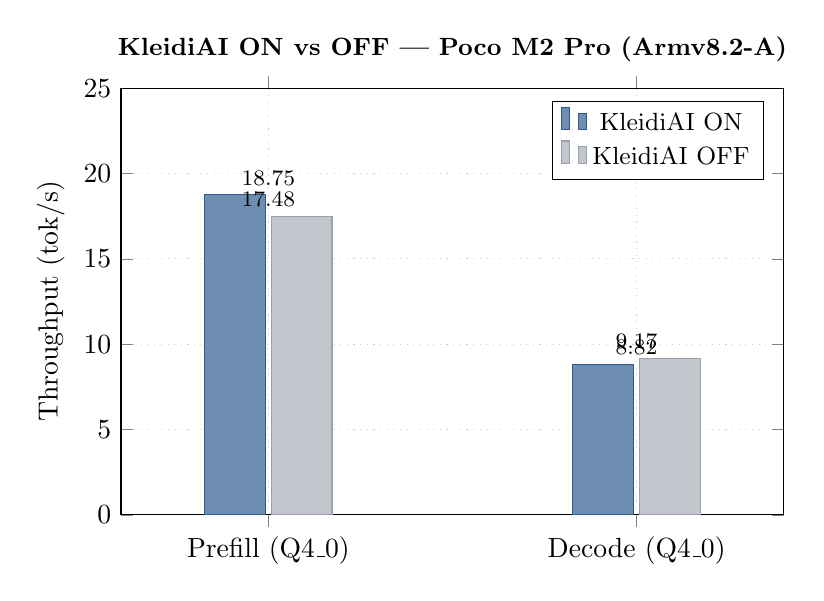
\begin{tikzpicture}
\begin{axis}[
  ybar, bar width=22pt,
  width=10cm, height=7cm,
  ylabel={Throughput (tok/s)},
  symbolic x coords={Prefill (Q4\_0), Decode (Q4\_0)},
  xtick=data,
  ymin=0, ymax=25,
  legend style={at={(0.97,0.97)}, anchor=north east, font=\small},
  enlarge x limits=0.4,
  nodes near coords, nodes near coords align=above,
  every node near coord/.style={font=\footnotesize},
  grid=major, grid style={dotted, gray!40},
  title={\textbf{KleidiAI ON vs OFF — Poco M2 Pro (Armv8.2-A)}},
  title style={font=\small\bfseries},
]
  \addplot[fill=blue!70, draw=blue] coordinates {
    (Prefill (Q4\_0), 18.75)
    (Decode (Q4\_0),   8.82)
  };
  \addplot[fill=inkfaint!60, draw=inkfaint] coordinates {
    (Prefill (Q4\_0), 17.48)
    (Decode (Q4\_0),   9.17)
  };
  \legend{KleidiAI ON, KleidiAI OFF}
\end{axis}
\end{tikzpicture}
\vspace{0.3em}

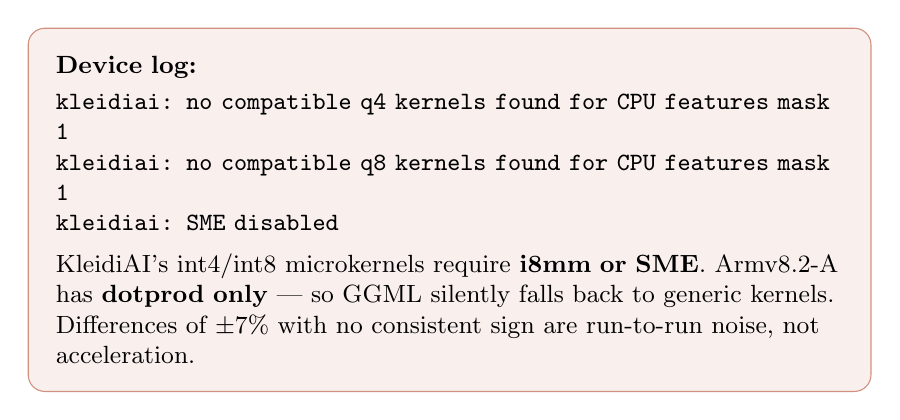
\begin{tikzpicture}
  \node[draw=red!60, fill=red!8, rounded corners=6pt,
        text width=10cm, align=left, inner sep=10pt, font=\small] {
    \textbf{Device log:}\\[2pt]
    \texttt{kleidiai: no compatible q4 kernels found for CPU features mask 1}\\
    \texttt{kleidiai: no compatible q8 kernels found for CPU features mask 1}\\
    \texttt{kleidiai: SME disabled}\\[4pt]
    KleidiAI's int4/int8 microkernels require \textbf{i8mm or SME}.
    Armv8.2-A has \textbf{dotprod only} — so GGML silently falls back to generic kernels.
    Differences of $\pm$7\% with no consistent sign are run-to-run noise, not acceleration.
  };
\end{tikzpicture}
\caption{\textbf{Diagram 3 — KleidiAI A/B Measurement.}
The headline finding: KleidiAI engages on i8mm/SME hardware, but not on Armv8.2-A
(dotprod only). Decode is marginally \emph{faster} with KleidiAI off — that is noise.
This cliff covers a large share of the global mid-range phone install base.}
\end{figure}

% ==============================================================
% DIAGRAM 4 — Thread Scaling & Decode Collapse
% ==============================================================
\begin{figure}[H]
\centering
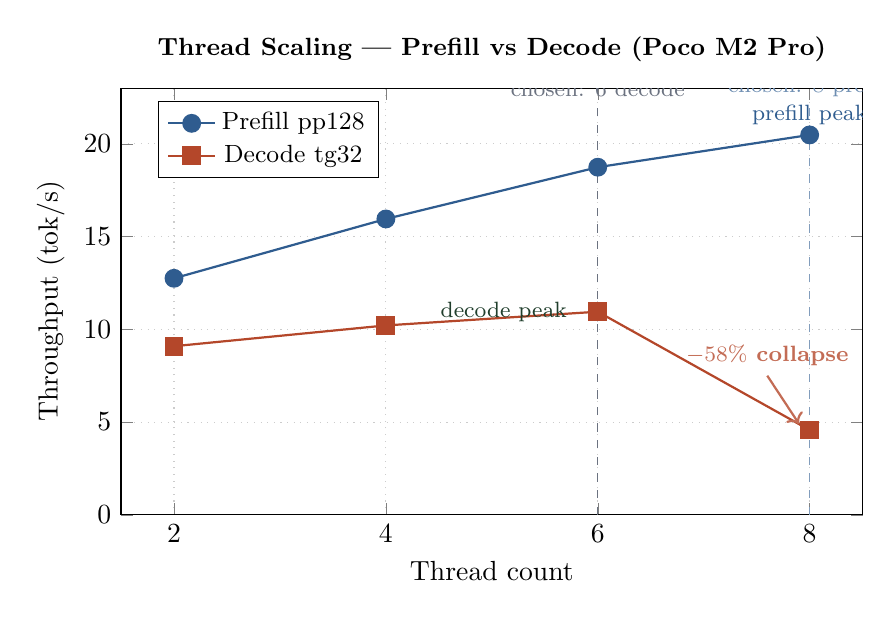
\begin{tikzpicture}
\begin{axis}[
  width=11cm, height=7cm,
  xlabel={Thread count}, ylabel={Throughput (tok/s)},
  xmin=1.5, xmax=8.5, ymin=0, ymax=23,
  xtick={2,4,6,8},
  legend style={at={(0.05,0.97)}, anchor=north west, font=\small},
  grid=major, grid style={dotted, gray!40},
  title={\textbf{Thread Scaling — Prefill vs Decode (Poco M2 Pro)}},
  title style={font=\small\bfseries},
  mark size=3pt,
]
  % prefill
  \addplot[color=blue, thick, mark=*, mark options={fill=blue}]
    coordinates {(2,12.75)(4,15.95)(6,18.74)(8,20.48)};
  \addlegendentry{Prefill pp128}

  % decode
  \addplot[color=red, thick, mark=square*, mark options={fill=red}]
    coordinates {(2,9.09)(4,10.21)(6,10.95)(8,4.57)};
  \addlegendentry{Decode tg32}

  % annotation: collapse
  \draw[->, red!80, thick] (axis cs:7.6,7.5)
    -- node[above, font=\footnotesize\bfseries, text=red!80, pos=0.0]
       {$-58\%$ collapse} (axis cs:7.9,4.9);

  % annotation: optima
  \node[font=\footnotesize, text=blue, anchor=south]
    at (axis cs:8, 20.48) {prefill peak};
  \node[font=\footnotesize, text=green!50!black, anchor=east]
    at (axis cs:5.8, 10.95) {decode peak};

  % vertical dashed: chosen config
  \draw[dashed, inksoft] (axis cs:6,0) -- (axis cs:6,22)
    node[above, font=\footnotesize, text=inksoft] {chosen: 6 decode};
  \draw[dashed, blue!60] (axis cs:8,0) -- (axis cs:8,22)
    node[above, font=\footnotesize, text=blue!70] {chosen: 8 prefill};
\end{axis}
\end{tikzpicture}
\caption{\textbf{Diagram 4 — Thread Scaling.}
Prefill (reading the prompt) is compute-bound and scales to 8 threads.
Decode (writing the answer) is memory-bandwidth-bound and \emph{collapses 58\%}
at 8 threads because the two fast A76 cores spend their time waiting at barriers
for the six slow A55 cores.
Cram uses \texttt{n\_threads\_batch=8}, \texttt{n\_threads=6} — the only app
configuration that takes advantage of both optima.}
\end{figure}

% ==============================================================
% DIAGRAM 5 — Prefill ≈ 2× Decode (vs GPU)
% ==============================================================
\begin{figure}[H]
\centering
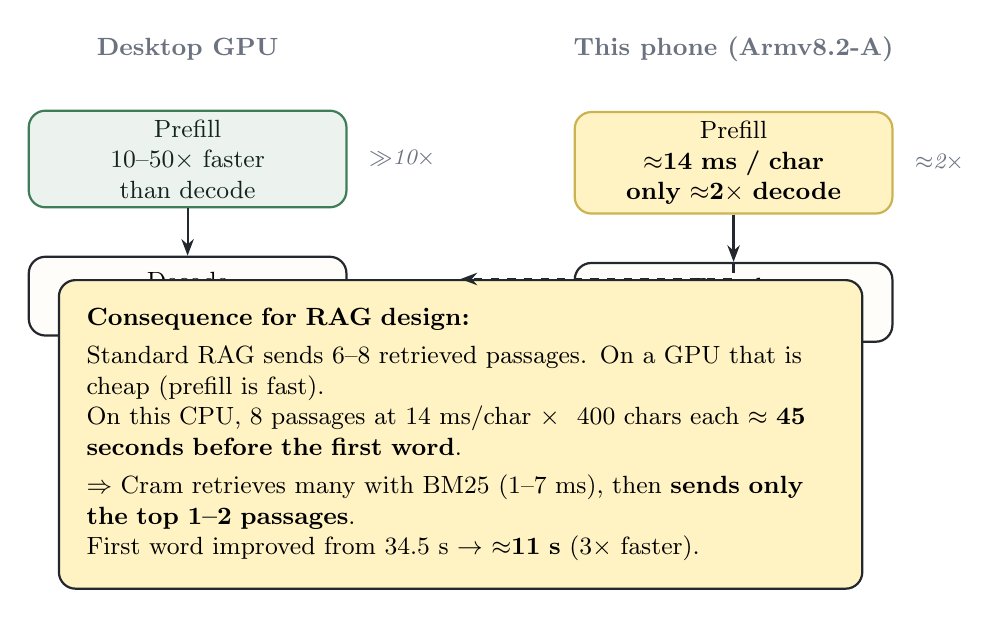
\begin{tikzpicture}[node distance=1cm]

  % GPU column
  \node[font=\bfseries\small, text=inksoft] (glabel) {Desktop GPU};
  \node[good, text width=3.8cm, below=0.5cm of glabel] (gpre)
    {Prefill\\10--50$\times$ faster\\than decode};
  \node[box, text width=3.8cm, below=0.6cm of gpre] (gdec)
    {Decode\\baseline};
  \draw[arr] (gpre) -- (gdec);
  \node[labl, right=0.15cm of gpre] {$\gg$10$\times$};

  % CPU column
  \node[font=\bfseries\small, text=inksoft, right=3.5cm of glabel] (clabel)
    {This phone (Armv8.2-A)};
  \node[warn, text width=3.8cm, below=0.5cm of clabel] (cpre)
    {Prefill\\\textbf{$\approx$14 ms / char}\\\textbf{only $\approx$2$\times$ decode}};
  \node[box, text width=3.8cm, below=0.6cm of cpre] (cdec)
    {Decode\\baseline};
  \draw[arr] (cpre) -- (cdec);
  \node[labl, right=0.15cm of cpre] {$\approx$2$\times$};

  % consequence box
  \node[draw=ink, thick, rounded corners=6pt, fill=ysoft,
        text width=9.5cm, align=left, inner sep=10pt, font=\small,
        below=1.5cm of $(gpre)!0.5!(cpre)$] (cons) {
    \textbf{Consequence for RAG design:}\\[3pt]
    Standard RAG sends 6--8 retrieved passages. On a GPU that is cheap (prefill is fast).\\
    On this CPU, 8 passages at 14 ms/char $\times$ ~400 chars each $\approx$ \textbf{45 seconds before the first word}.\\[3pt]
    $\Rightarrow$ Cram retrieves many with BM25 (1--7 ms), then \textbf{sends only the top 1--2 passages}.\\
    First word improved from 34.5 s $\to$ \textbf{$\approx$11 s} (3$\times$ faster).
  };

  \draw[darr] (cpre.south) |- (cons.north);

\end{tikzpicture}
\caption{\textbf{Diagram 5 — Why the Prefill Ratio Changes Everything.}
On a GPU, prefill is 10--50$\times$ faster than decode, so sending many passages is free.
On this CPU, prefill runs at only $\approx$2$\times$ decode speed ($\approx$14 ms/char),
making the standard ``stuff the context'' RAG approach unusably slow.}
\end{figure}

% ==============================================================
% DIAGRAM 6 — CPU Cluster Architecture (Big.LITTLE)
% ==============================================================
\begin{figure}[H]
\centering
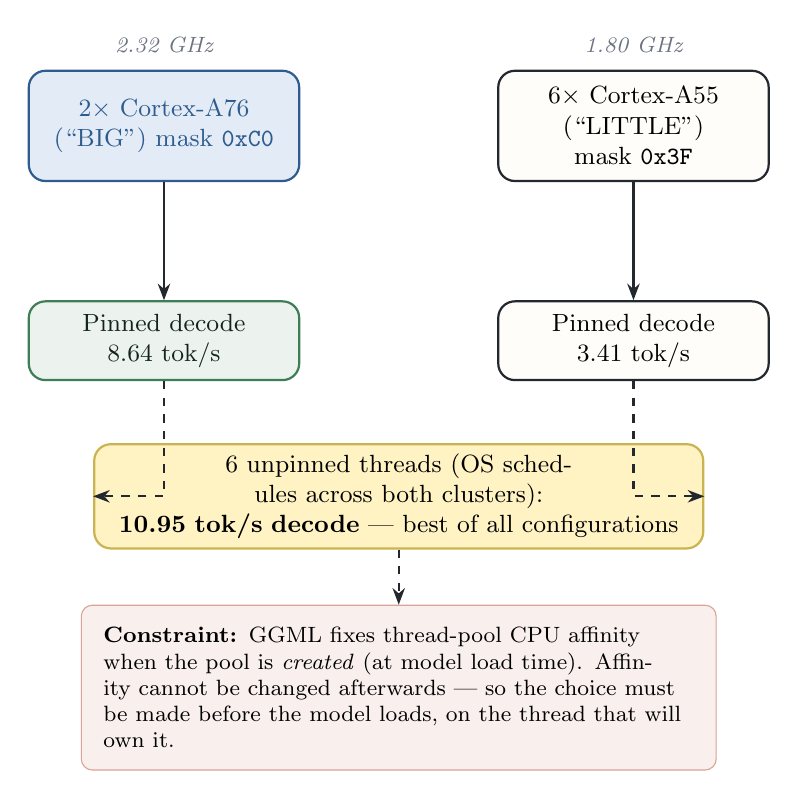
\begin{tikzpicture}

  % Big cluster
  \node[accent, text width=3.2cm, minimum height=1.4cm]
    (big) {2$\times$ Cortex-A76\\(``BIG'') mask \texttt{0xC0}};

  % Little cluster
  \node[box, text width=3.2cm, minimum height=1.4cm, right=2.5cm of big]
    (lit) {6$\times$ Cortex-A55\\(``LITTLE'') mask \texttt{0x3F}};

  % decode result
  \node[good, text width=3.2cm, below=1.5cm of big] (bdec)
    {Pinned decode\\8.64 tok/s};
  \node[box,  text width=3.2cm, below=1.5cm of lit]  (ldec)
    {Pinned decode\\3.41 tok/s};

  % unpinned result
  \node[warn, text width=7.5cm, below=1.3cm of $(bdec)!0.5!(ldec)$] (unpin)
    {6 unpinned threads (OS schedules across both clusters):\\
     \textbf{10.95 tok/s decode} — best of all configurations};

  \draw[arr] (big) -- (bdec);
  \draw[arr] (lit) -- (ldec);
  \draw[darr] (bdec.south) |- (unpin.west);
  \draw[darr] (ldec.south) |- (unpin.east);

  % note
  \node[draw=red!50, fill=red!8, rounded corners=4pt,
        text width=7.5cm, align=left, inner sep=8pt, font=\footnotesize,
        below=0.7cm of unpin] (note) {
    \textbf{Constraint:} GGML fixes thread-pool CPU affinity when the pool is \emph{created}
    (at model load time). Affinity cannot be changed afterwards — so the choice must
    be made before the model loads, on the thread that will own it.
  };
  \draw[darr] (unpin) -- (note);

  % frequency labels
  \node[labl, above=0.1cm of big] {2.32 GHz};
  \node[labl, above=0.1cm of lit] {1.80 GHz};

\end{tikzpicture}
\caption{\textbf{Diagram 6 — Big.LITTLE Cluster Comparison.}
Counter-intuitively, 6 unpinned threads outperform 2 pinned big-core threads (10.95 vs 8.64 tok/s)
because the little cores contribute real work at this model size.
The 2$\times$ A76 still beat all 6$\times$ A55 in a fair cluster-vs-cluster comparison (8.64 vs 3.41).}
\end{figure}

% ==============================================================
% DIAGRAM 7 — App Screen Flow (the core loop)
% ==============================================================
\begin{figure}[H]
\centering
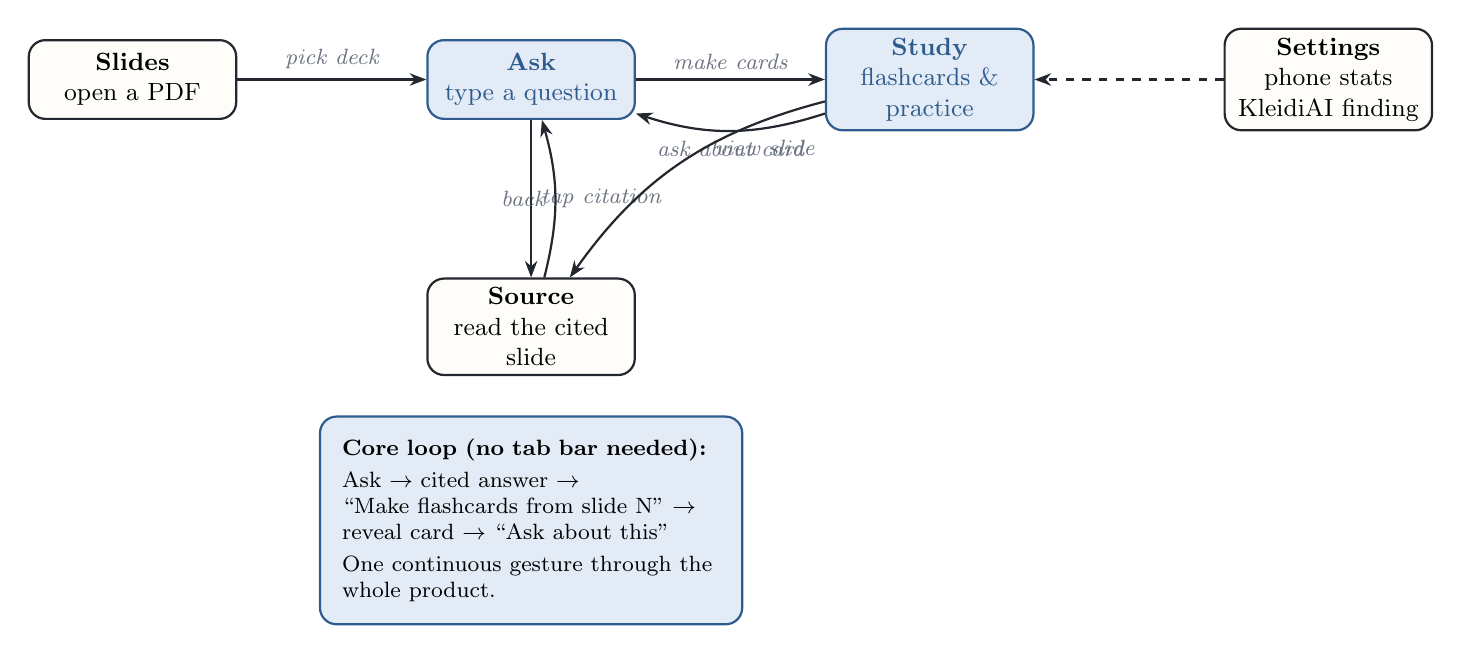
\begin{tikzpicture}[node distance=1.4cm and 2.4cm]

  % screens
  \node[box, text width=2.4cm] (slides) {\textbf{Slides}\\\small open a PDF};
  \node[accent, text width=2.4cm, right=of slides] (ask)
    {\textbf{Ask}\\\small type a question};
  \node[accent, text width=2.4cm, right=of ask] (study)
    {\textbf{Study}\\\small flashcards \&\\practice};
  \node[box, text width=2.4cm, below=2cm of ask] (source)
    {\textbf{Source}\\\small read the cited\\slide};
  \node[box, text width=2.4cm, right=of study] (settings)
    {\textbf{Settings}\\\small phone stats\\KleidiAI finding};

  % main flow arrows
  \draw[arr] (slides) -- node[labl,above]{pick deck} (ask);
  \draw[arr] (ask)    -- node[labl,above]{make cards} (study);
  \draw[arr, bend left=18] (study) to
    node[labl,below, pos=0.5]{ask about card} (ask);

  % citation cross-links
  \draw[arr] (ask)   -- node[labl,right]{tap citation} (source);
  \draw[arr, bend right=20] (study) to
    node[labl, right, pos=0.4]{view slide} (source);
  \draw[arr, bend right=15] (source) to
    node[labl, left, pos=0.5]{back} (ask);

  % settings
  \draw[darr] (settings.west) -- (study.east);

  % the core loop callout
  \node[draw=blue, thick, rounded corners=6pt, fill=bluesoft,
        text width=4.8cm, align=left, inner sep=8pt, font=\footnotesize,
        below=0.5cm of source] (loop) {
    \textbf{Core loop (no tab bar needed):}\\[2pt]
    Ask $\to$ cited answer $\to$\\
    ``Make flashcards from slide N'' $\to$\\
    reveal card $\to$ ``Ask about this''\\[2pt]
    One continuous gesture through the whole product.
  };

\end{tikzpicture}
\caption{\textbf{Diagram 7 — App Screen Flow.}
The five tabs are connected by cross-links so the user never needs to navigate manually.
Ask is the front door; Study is the payoff; Source is the proof.
Settings is judge-facing — it displays the KleidiAI finding on \emph{the judge's own phone}.}
\end{figure}

% ==============================================================
% DIAGRAM 8 — Memory \& Context Budget Strategy
% ==============================================================
\begin{figure}[H]
\centering
\begin{tikzpicture}

  % Phone memory bar
  \node[font=\bfseries\small, text=ink] at (0, 3.3) {Available RAM — Poco M2 Pro ($\approx$5.4 GB)};

  % stacked bar
  \fill[blue!70]   (0,2.5) rectangle (4.2, 3.0)
    node[midway, font=\footnotesize\bfseries, text=white] {Model weights (Q4\_0) $\approx$800 MB};
  \fill[green!50]  (4.2,2.5) rectangle (5.8, 3.0)
    node[midway, font=\footnotesize, text=white] {KV cache};
  \fill[yellow!70] (5.8,2.5) rectangle (7.2, 3.0)
    node[midway, font=\footnotesize, text=ink] {OS};
  \fill[inkfaint!40] (7.2,2.5) rectangle (10, 3.0)
    node[midway, font=\footnotesize, text=ink] {free headroom};
  \draw[ink, thick] (0,2.5) rectangle (10,3.0);

  % n_ctx annotation
  \draw[{Stealth[length=5pt]}-{Stealth[length=5pt]}, blue, thick]
    (4.2, 2.1) -- (5.8, 2.1)
    node[midway, below, font=\footnotesize, text=blue]
    {\texttt{n\_ctx=2048} (not 131072!)};
  \draw[dashed, blue!50] (4.2,2.5) -- (4.2,2.15);
  \draw[dashed, blue!50] (5.8,2.5) -- (5.8,2.15);

  \node[draw=red!60, fill=red!8, rounded corners=5pt,
        text width=9cm, align=left, inner sep=8pt, font=\footnotesize,
        below=0.4cm of $(0,2.1)$] (warn2) {
    \textbf{Without \texttt{-c 2048}:} Llama 3.2's trained context is 131\,072 tokens.
    Defaulting to it allocates a multi-GB KV cache.
    Android's Low Memory Killer terminates the app — or the phone reboots.
    \texttt{-c 2048} is the single most important flag in the entire codebase.
  };

  % Char budget diagram
  \node[font=\bfseries\small, text=ink, below=0.5cm of warn2.south west, anchor=north west]
    (blabel) {Prompt character budget (greedy allocation):};

  \node[below=0.3cm of blabel.south west, anchor=north west] (bbase) {};

  \fill[blue!70]   (0,-2.2) rectangle (5.5,-1.7)
    node[midway, font=\footnotesize\bfseries, text=white] {Top passage (fills first)};
  \fill[inkfaint!50] (5.5,-2.2) rectangle (8.5,-1.7)
    node[midway, font=\footnotesize, text=white] {Runner-up (remainder)};
  \fill[yellow!70]   (8.5,-2.2) rectangle (10,-1.7)
    node[midway, font=\footnotesize, text=ink] {Q+A};
  \draw[ink, thick]  (0,-2.2) rectangle (10,-1.7);

  \draw[{Stealth[length=4pt]}-{Stealth[length=4pt]}, ink]
    (0,-2.5) -- (10,-2.5) node[midway, below, font=\footnotesize]
    {char budget $\geq 900$ chars (floor raised after hallucination incident)};

\end{tikzpicture}
\caption{\textbf{Diagram 8 — Memory and Context Budget.}
The KV cache size is explicitly capped at \texttt{n\_ctx=2048}.
Within the budget, the best-matching passage is allocated first; the runner-up takes
whatever remains. The 900-char floor was added after the model \emph{invented}
two of the four Coffman conditions when the budget was squeezed to 400 chars for speed.}
\end{figure}

% ==============================================================
% DIAGRAM 9 — Startup Calibration Flow
% ==============================================================
\begin{figure}[H]
\centering
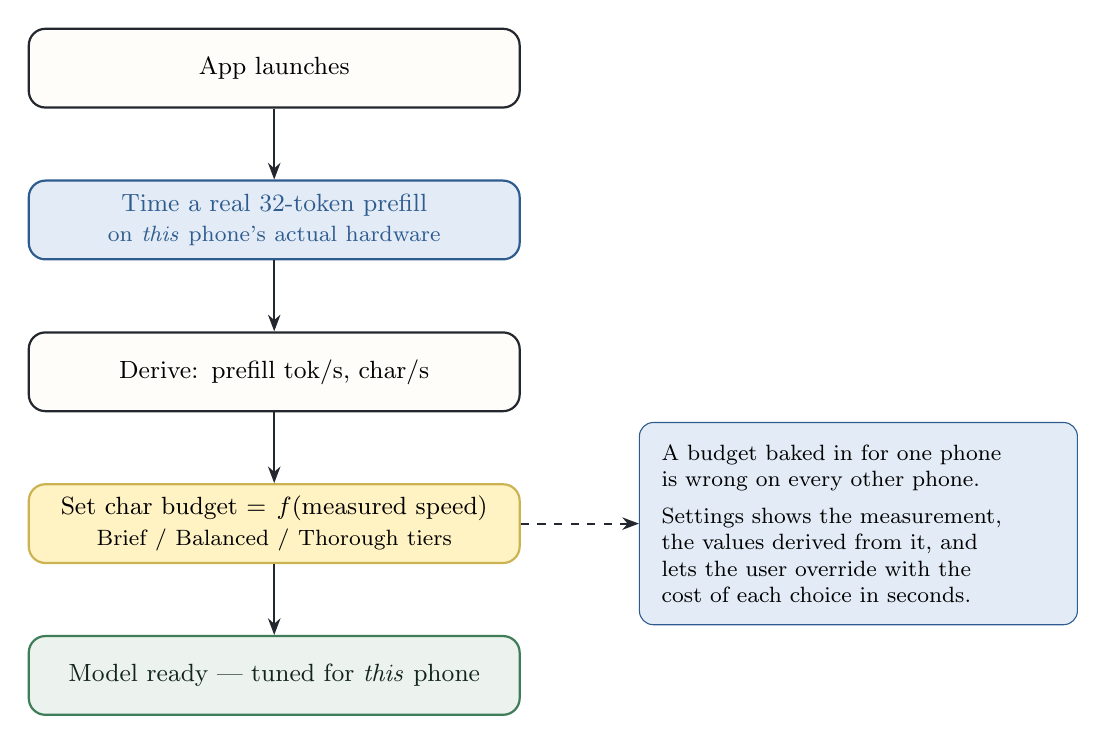
\begin{tikzpicture}[node distance=0.9cm]

  \node[box, text width=6cm] (boot)
    {App launches};
  \node[accent, text width=6cm, below=of boot] (cal)
    {Time a real 32-token prefill\\{\footnotesize on \textit{this} phone's actual hardware}};
  \node[box, text width=6cm, below=of cal] (tps)
    {Derive: prefill tok/s, char/s};
  \node[warn, text width=6cm, below=of tps] (budget)
    {Set char budget $= f$(measured speed)\\{\footnotesize Brief / Balanced / Thorough tiers}};
  \node[good, text width=6cm, below=of budget] (ready)
    {Model ready — tuned for \textit{this} phone};

  \foreach \a/\b in {boot/cal, cal/tps, tps/budget, budget/ready}
    \draw[arr] (\a) -- (\b);

  \node[draw=blue, fill=bluesoft, rounded corners=5pt,
        text width=5cm, align=left, inner sep=8pt, font=\footnotesize,
        right=1.5cm of budget] (side) {
    A budget baked in for one phone\\
    is wrong on every other phone.\\[4pt]
    Settings shows the measurement,\\
    the values derived from it, and\\
    lets the user override with the\\
    cost of each choice in seconds.
  };
  \draw[darr] (budget.east) -- (side.west);

\end{tikzpicture}
\caption{\textbf{Diagram 9 — Startup Calibration.}
At first launch, Cram times a real prefill pass and sets its own prompt-budget
to match \emph{this specific phone's} throughput. A budget measured on a Snapdragon 720G
would be wrong on a Dimensity 920 — so the app measures rather than assumes.}
\end{figure}

\end{document}
